% ****** Start of file aipsamp.tex ******
%
%   This file is part of the AIP files in the AIP distribution for REVTeX 4.
%   Version 4.1 of REVTeX, October 2009
%
%   Copyright (c) 2009 American Institute of Physics.

% Use this file as a source of example code for your aip document.
% Use the file aiptemplate.tex as a template for your document.
\documentclass[%
	aip,
	jmp,%
	amsmath,amssymb,
	%preprint,%
	reprint,%
	%author-year,%
	%author-numerical,%
]{revtex4-1}
%\extrafloats{1000}
\usepackage{morefloats}% Include figure files
\usepackage{graphicx}% Include figure files
\usepackage{grffile}
\usepackage{afterpage}
\usepackage{dcolumn}% Align table columns on decimal point
\usepackage{bm}% bold math
%\usepackage[mathlines]{lineno}% Enable numbering of text and display math
%\linenumbers\relax % Commence numbering lines
\usepackage{multirow}
\usepackage{color} % for the notes
\usepackage{etex}
\reserveinserts{58}
%\usepackage{morefloats}
\usepackage{hyperref}
\usepackage{xcolor}
\usepackage{amsmath}
\hypersetup{
	colorlinks,
	linkcolor={red!50!black},
	citecolor={blue!50!black},
	urlcolor={blue!80!black}
}

\usepackage{xr}
\externaldocument{supportingInformation}
\maxdeadcycles=1000

\usepackage{placeins}
\begin{document}

\preprint{XXXXX (preprint)}

%\title[Evolution of interaction networks]{On the evolution of interaction networks: primitive typology of vertex, prominence of measures and activity statistics}% Force line breaks with \\
%\title[Evolution of interaction networks]{On the evolution of interaction networks: a primitive typology of vertex}% Force line breaks with \\
%\title[Stability of interaction networks]{Stability in human interaction networks: sector relative sizes, prominence of topological measures and time activity statistics.}% Force line breaks with \\
%\title[Stability in human interaction networks]{Sector relative sizes and topological metrics time stability in human interaction networks}% Force line breaks with \\
\title[Distances between histograms]{A distance metric between histograms
through the the Kolmogorov-Smirnov test statistic: specification, measures reference and example uses}% Force line breaks with \\
\author{Renato Fabbri}%
\homepage{http://ifsc.usp.br/~fabbri/}
\email{fabbri@usp.br}
\affiliation{ 
	S\~ao Carlos Institute of Physics, University of S\~ao Paulo (IFSC/USP),
	PO Box 369, 13560-970, S\~ao Carlos, SP, Brazil %\\This line break forced with \textbackslash\textbackslash
}

\date{\today}% It is always \today, today,
%  but any date may be explicitly specified

\begin{abstract}
This document presents reference values for a distance metric
derived from the Kolmogorov-Smirnov test statistic $D_{F,F'}$.
Each measure of $D_{F,F'}$ is a distance between two histograms,
which is normalized by the number of observations in each sample
to yield the $c$ statistic, which can be mapped to p-values, i.e. values for which 
higher levels of significance $\alpha>c(\alpha)$ implies the rejection of the null hypothesis.
Benchmarks for the implementation are delivered by comparing samples from known distributions.
Pattern examples in real data enables further
insight in the robustness and power of $c$.
\end{abstract}

\pacs{05.10-a,}% PACS, the Physics and Astronomy
\keywords{Kolmogorov-Smirnov test, statistic, benchmark, distance measure, histogram}
\maketitle


\tableofcontents


\section{Introduction}\label{sec:intro}

% $D_{n,n'}$
%depicted in Figure~\ref{fig:kolms}


Be $F$ and $F'$ two empirical cumulative distributions,
where $n$ and $n'$ are the number of observations on each sample.
The two-sample Kolmogorov-Smirnov test rejects the null hypothesis
that the histograms are the outcome of the same underlying distribution
if:
\begin{equation}\label{eq:ks}
D_{F,F'} > c(\alpha)\sqrt{\frac{n+n'}{nn'}}
\end{equation}

\noindent where $D_{F,F'}=sup_x[F-F']$ as in Figure~\ref{fig:dnn}
and $c(\alpha)$ is related to the level of significance $\alpha$ by:

\begin{table}[h!]
\centering
\begin{tabular}{|l||c|c|c|c|c|c|}\hline
$\alpha$    & 0.1  & 0.05 & 0.025 & 0.01 & 0.005 & 0.001 \\\hline
$c(\alpha)$ & 1.22 & 1.36 & 1.48  & 1.63 & 1.73  & 1.95  \\\hline
\end{tabular}
\end{table}

If distributions are drawn from empirical data, $D_{F,F'}$ is given as are $n$ and $n'$.
All terms in equation~\ref{eq:ks} are positive and $c(\alpha)$ can be isolated:

\begin{equation}\label{eq:ks2}
	c(\alpha) < \frac{D_{n,n'}}{\sqrt{\frac{n+n'}{nn'}}} = c
\end{equation}

%Tables~\ref{tab:kolSub}-\ref{tab:kolPctInter} are populated with values for $c'(\alpha)$
When $c$ is high, low values of $\alpha$ favor rejecting the null hypothesis.
In fact, $c$ can be normalized to yield p-values.

\begin{figure}[!h]
	\centering
	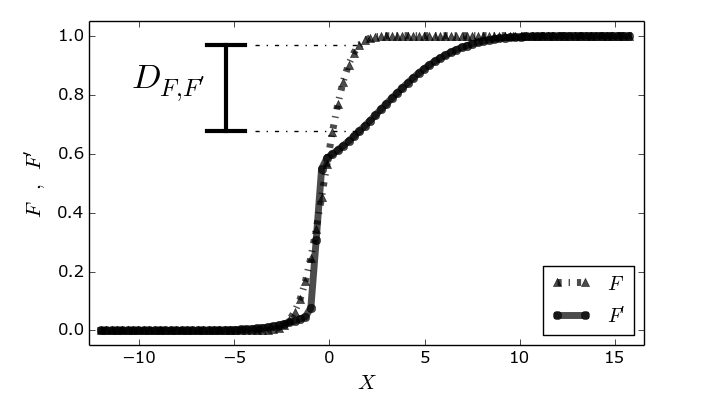
\includegraphics[width=0.44\textwidth]{figs/Dnn}
	\caption{The Kolmogorov-Smirnov statistic $D_{F,F'}$: the maximum difference between
		two cumulative distribution functions.}
	\label{fig:dnn}
\end{figure}

Hight values of $c$ favor rejecting the null hypothesis.
For example, if the significance level is $\alpha=0.01$,
then $c$ greater than $1.7$
implies the rejection of the null hypothesis and
suggests that $F$ and $F'$
are outcomes of different distributions.
Of core importance in this study is to regard the $c$ statistic
as a measure of distance between both distributions~\cite{kolm}.
The main contribution of the following sections is the
explicit display of reference values of $c$
from which one might derive knowledge from
measures or even from a single value of $c$.

%\subsection{Workarounds}
%The Kolmogorov-Smirnov test is robust,
%but data often fall into the cases where
%it is not guaranteed to be valid.
%In order to make the example analysis,
%the empirical density functions are built from discrete data.
%
%as we fall into two of these.
%
% z-score
% discrete
% formulação com max(f-x,x-f2)

%If the number of elements ($n$ and $n'$)
%in each sample are bellow 50.

\subsection{Philosophical and technological note}
Difference and equivalence is of central role in human cognition,
philosophy and science.
This fact is so deeply recognized that thinkers often reduce
thought to classifications, e.g. through the
mathematical concept of equivalence classes~\cite{deleuze}.
Histograms are very immediate and informative
roughly wherever there is a phenomenon of interest which can yield measurements.
This present document should enable conclusions to be drawn about 
the equivalence (and difference)
of the processes underlying sets of measurements for a very
broad range of phenomena.
The following tables 
validate the mathematical framework
and the software implementation.

\subsection{Document outline}
Section~\ref{sec:simulations} exposes reference values drawn from simulations.
Section~\ref{sec:empirical} exemplifies the use of such reference values
to make sense of phenomena.
Section~\ref{sec:conc} holds final remarks.
Software and data specification are given in Appendix~\ref{ap:soft}.

\section{References through simulations}\label{sec:simulations}
On every case, values of $c$ are given for simulations involving
at least normal, uniform, Weibull and power function distributions.
The rendering of this article is automated to ease changes in
the settings with which the results are reported.
\input{aux/preambule1}

\subsection{When the null hypothesis is true}
If the null hypothesis is true, than the number
of rejections of the null hypothesis (that is: $c>c(\alpha)$)
in $N_c$ comparisons should not exceed $\alpha N_c$.
To verify this, let $C=\{c_i\}$ be a set of $c$ measures,
and $C(\alpha)=\{c : c>c(\alpha)\}$.
Be $|C(\alpha)|$ the cardinality of $C(\alpha)$,
i.e. the number of comparisons in which the two-sample Kolmogorov-Smirnov
test rejects the null hypothesis for a given $\alpha$.
This section reports that
$|C(\alpha)|$ very rarely exceeds $\alpha N_c$,
for all probability distributions and settings.
Also important are that
$c>c(\alpha)$ in many cases
and that the tabulated $\alpha$ values
are also good estimates of the upper limit
of the frequency of such an event.

%\begin{itemize}
%	\item $c'>c(\alpha)$ in many cases, and $\alpha N_c$ is a good upper limit to keep in mind.
%	\item 
%\end{itemize}

% Input tables
% any plot? If std is ~stable, plots of the mean of c~(\alpha) are compact and informative
\begin{table}[h!]
\begin{center}
\begin{tabular}{| l | c | c | c | c | c |}\hline
$\alpha N_c$ & $\alpha$ & $c(\alpha)$ & $|C_1(\alpha)|$ & $|C_2(\alpha)|$ & $|C_3(\alpha)|$ \\\hline\hline
10.0 & 0.100 & 1.22 & 7 & 10 & 8 \\\hline
5.0 & 0.050 & 1.36 & 5 & 3 & 4 \\\hline
2.5 & 0.025 & 1.48 & 3 & 1 & 3 \\\hline
1.0 & 0.010 & 1.63 & 0 & 1 & 3 \\\hline
0.5 & 0.005 & 1.73 & 0 & 0 & 1 \\\hline
0.1 & 0.001 & 1.95 & 0 & 0 & 0 \\\hline
\end{tabular}
\caption{The theoretical maximum number $\alpha N_c$ of rejections
of the null hypothesis for significance levels $\alpha$.
The $c_1$ values were calculated using simulations of normal distributions with $\mu=0$ and $\sigma=1$.
The $c_2$ values were calculated using simulations of normal distributions with $\mu=3$ and $\sigma=2$.
The $c_3$ values were calculated using simulations of normal distributions with $\mu=6$ and $\sigma=3$.
Over all $N_c$ comparisons,
 $\mu(c_1)=0.8218$ and $\sigma(c_1)=0.2515$,
 $\mu(c_2)=0.7811$ and $\sigma(c_2)=0.2748$,
 $\mu(c_3)=0.8365$ and $\sigma(c_3)=0.2523$ .
}
\end{center}
\end{table}
\begin{table}[h!]
\begin{center}
\begin{tabular}{| l | c | c | c | c | c |}\hline
$\alpha N_c$ & $\alpha$ & $c(\alpha)$ & $|C_1(\alpha)|$ & $|C_2(\alpha)|$ & $|C_3(\alpha)|$ \\\hline\hline
10.0 & 0.100 & 1.22 & 9 & 8 & 8 \\\hline
5.0 & 0.050 & 1.36 & 4 & 3 & 3 \\\hline
2.5 & 0.025 & 1.48 & 1 & 2 & 2 \\\hline
1.0 & 0.010 & 1.63 & 0 & 0 & 2 \\\hline
0.5 & 0.005 & 1.73 & 0 & 0 & 1 \\\hline
0.1 & 0.001 & 1.95 & 0 & 0 & 0 \\\hline
\end{tabular}
\caption{The theoretical maximum number $\alpha N_c$ of rejections
of the null hypothesis for critical values of $\alpha$.
The $c_1$ values were calculated using simulations of uniform distributions within $[0,1)$.
The $c_2$ values were calculated using simulations of uniform distributions within $[2,6)$.
The $c_3$ values were calculated using simulations of uniform distributions with $\mu=4$ and $\sigma=10$.
Over all $N_c$ comparisons,
 $\mu(c_1)=0.8616$ and $\sigma(c_1)=0.2291$,
 $\mu(c_2)=0.8345$ and $\sigma(c_2)=0.2492$,
 $\mu(c_3)=0.8086$ and $\sigma(c_3)=0.2740$ .
}
\end{center}
\end{table}
\begin{table}[h!]
\begin{center}
\begin{tabular}{| l | c | c | c | c | c | c |}\hline
$\alpha N_c$ & $\alpha$ & $c(\alpha)$ & $|C_1(\alpha)|$ & $|C_2(\alpha)|$ & $|C_3(\alpha)|$ & $|C_4(\alpha)|$ \\\hline\hline
10.0 & 0.100 & 1.22 & 0 & 4 & 3 & 8 \\\hline
5.0 & 0.050 & 1.36 & 0 & 0 & 1 & 3 \\\hline
2.5 & 0.025 & 1.48 & 0 & 0 & 0 & 0 \\\hline
1.0 & 0.010 & 1.63 & 0 & 0 & 0 & 0 \\\hline
0.5 & 0.005 & 1.73 & 0 & 0 & 0 & 0 \\\hline
0.1 & 0.001 & 1.95 & 0 & 0 & 0 & 0 \\\hline
\end{tabular}
\caption{The theoretical maximum number $\alpha N_c$ of rejections
of the null hypothesis for critical values of $\alpha$.
The $c_1$ values were calculated using simulations of 1-parameter Weibull distributions with $a=0.1$.
The $c_2$ values were calculated using simulations of 1-parameter Weibull distributions with $a=2$.
The $c_3$ values were calculated using simulations of 1-parameter Weibull distributions with $a=4$.
Over all $N_c$ comparisons,
The $N_o$ values of $c_4$ were calculated using simulations of
 1-parameter Weibull distributions with $a=6$.
Over all $N_c$ comparisons,
 $\mu(c_1)=0.0655$ and $\sigma(c_1)=0.0376$,
 $\mu(c_2)=0.7053$ and $\sigma(c_2)=0.2261$,
 $\mu(c_3)=0.6905$ and $\sigma(c_3)=0.2460$ .
 $\mu(c_4)=0.7596$ and $\sigma(c_4)=0.2644$ .
}
\end{center}
\end{table}
\begin{table}[h!]
\begin{center}
\begin{tabular}{| l | c | c | c | c | c | c | c |}\hline
$\alpha N_c$ & $\alpha$ & $c(\alpha)$ & $|C_1(\alpha)|$ & $|C_2(\alpha)|$ & $|C_3(\alpha)|$ & $|C_4(\alpha)|$ & $|C_5(\alpha)|$ \\\hline\hline
10.0 & 0.100 & 1.22 & 6 & 12 & 12 & 9 & 7 \\\hline
5.0 & 0.050 & 1.36 & 6 & 3 & 5 & 4 & 2 \\\hline
2.5 & 0.025 & 1.48 & 2 & 0 & 1 & 2 & 1 \\\hline
1.0 & 0.010 & 1.63 & 1 & 0 & 1 & 1 & 0 \\\hline
0.5 & 0.005 & 1.73 & 1 & 0 & 1 & 1 & 0 \\\hline
0.1 & 0.001 & 1.95 & 0 & 0 & 0 & 0 & 0 \\\hline
\end{tabular}
\caption{The theoretical maximum number $\alpha N_c$ of rejections
of the null hypothesis for critical values of $\alpha$.
The $c_1$ values were calculated using simulations of power functions distributions with $a=0.3$.
The $c_2$ values were calculated using simulations of power functions distributions with $a=1$.
The $c_3$ values were calculated using simulations of power functions distributions with $a=2$.
The $c_4$ values were calculated using simulations of power functions distributions with $a=3$.
The $c_5$ values were calculated using simulations of power functions distributions with $a=4$.
Over all $N_c$ comparisons,
 $\mu(c_1)=0.8253$ and $\sigma(c_1)=0.2697$,
 $\mu(c_2)=0.8470$ and $\sigma(c_2)=0.2557$,
 $\mu(c_3)=0.8799$ and $\sigma(c_3)=0.2588$ .
 $\mu(c_4)=0.8278$ and $\sigma(c_4)=0.2637$ .
 $\mu(c_5)=0.7795$ and $\sigma(c_5)=0.2364$ .
}
\end{center}
\end{table}

\FloatBarrier
\subsection{When the null hypothesis if false}
The null hypothesis is always false for a sufficiently small
significance level $\alpha$.
In this section,
each table holds a set comparisons between two samples:
one sample is generated through a
fixed distribution while the other
sample is modified in each comparison.
The comparison is repeated $N_c$ times.
The measures on $c$ chosen to report the results are:
the mean $\mu(c)$, the standard deviation $\sigma(c)$,
the median $m(c)$,
the  fraction
$\overline{C(\alpha)}=\frac{|C(\alpha)|}{N_c}$
of rejection of the null hypothesis given the significance level $\alpha$.
The null hypothesis is true in the boldface lines.

\begin{table*}[h!]
\begin{center}
\begin{tabular}{| l | c | c | c | c | c | c | c | c | c | c | c |}\hline
$\sigma$ & $\mu(c)$ & $\sigma(c)$ & m(c) & min(c) & max(c) & $\overline{C(0.1)}$ & $\overline{C(0.05)}$ & $\overline{C(0.025)}$ & $\overline{C(0.01)}$ & $\overline{C(0.005)}$ & $\overline{C(0.001)}$ \\\hline\hline
0.5 & 3.965 & 0.309 & 3.958 & 3.354,3.421,3.444 & 4.606,4.696,4.763  & 1.000  & 1.000  & 1.000  & 1.000  & 1.000  & 1.000 \\\hline
0.6 & 3.072 & 0.276 & 3.075 & 2.348,2.549,2.571 & 3.667,3.712,3.913  & 1.000  & 1.000  & 1.000  & 1.000  & 1.000  & 1.000 \\\hline
0.7 & 2.287 & 0.243 & 2.292 & 1.632,1.766,1.834 & 2.795,2.817,2.952  & 1.000  & 1.000  & 1.000  & 1.000  & 0.990  & 0.910 \\\hline
0.8 & 1.718 & 0.263 & 1.699 & 1.118,1.118,1.185 & 2.214,2.326,2.393  & 0.960  & 0.920  & 0.830  & 0.650  & 0.440  & 0.220 \\\hline
0.9 & 1.131 & 0.290 & 1.129 & 0.537,0.559,0.626 & 1.789,1.834,1.901  & 0.350  & 0.190  & 0.110  & 0.080  & 0.040  & 0.000 \\\hline
{\bf 1.0} & {\bf 0.847} & {\bf 0.275} & {\bf 0.805} & {\bf 0.402,0.447,0.447} & {\bf 1.565,1.588,1.632} & {\bf 0.110} & {\bf 0.070} & {\bf 0.040} & {\bf 0.010} & {\bf 0.000} & {\bf 0.000} \\\hline
1.1 & 1.023 & 0.252 & 1.006 & 0.537,0.581,0.626 & 1.655,1.699,1.722  & 0.210  & 0.090  & 0.040  & 0.030  & 0.000  & 0.000 \\\hline
1.2 & 1.450 & 0.292 & 1.465 & 0.648,0.693,0.760 & 1.945,1.990,1.990  & 0.760  & 0.650  & 0.480  & 0.260  & 0.180  & 0.020 \\\hline
1.3 & 1.792 & 0.250 & 1.766 & 1.163,1.163,1.297 & 2.303,2.393,2.437  & 0.980  & 0.960  & 0.900  & 0.790  & 0.560  & 0.250 \\\hline
1.4 & 2.179 & 0.276 & 2.180 & 1.543,1.610,1.677 & 2.728,2.817,3.086  & 1.000  & 1.000  & 1.000  & 0.980  & 0.970  & 0.790 \\\hline
1.5 & 2.542 & 0.288 & 2.527 & 1.923,1.923,1.923 & 3.153,3.466,3.578  & 1.000  & 1.000  & 1.000  & 1.000  & 1.000  & 0.970 \\\hline
1.6 & 2.863 & 0.258 & 2.862 & 2.303,2.370,2.393 & 3.354,3.511,3.533  & 1.000  & 1.000  & 1.000  & 1.000  & 1.000  & 1.000 \\\hline
1.7 & 3.174 & 0.259 & 3.164 & 2.683,2.706,2.706 & 3.712,3.824,3.846  & 1.000  & 1.000  & 1.000  & 1.000  & 1.000  & 1.000 \\\hline
1.8 & 3.424 & 0.287 & 3.399 & 2.885,2.907,2.907 & 4.092,4.114,4.226  & 1.000  & 1.000  & 1.000  & 1.000  & 1.000  & 1.000 \\\hline
1.9 & 3.743 & 0.258 & 3.712 & 3.198,3.265,3.309 & 4.360,4.494,4.562  & 1.000  & 1.000  & 1.000  & 1.000  & 1.000  & 1.000 \\\hline
2.0 & 4.027 & 0.287 & 4.014 & 3.421,3.511,3.533 & 4.696,4.696,4.740  & 1.000  & 1.000  & 1.000  & 1.000  & 1.000  & 1.000 \\\hline
\end{tabular}
\caption{Measurements of $c$ through simulations
with normal distributions.
One normal distribution is fixed, with $\mu=0$ and $\sigma=1$,
and compared agaist normal distributions with $\mu=0$
and different values of $\sigma$.}
\end{center}
\end{table*}
\begin{table*}[h!]
\begin{center}
\begin{tabular}{| l | c | c | c | c | c | c | c | c | c | c | c |}\hline
$\mu$ & $\mu(c)$ & $\sigma(c)$ & m(c) & min(c) & max(c) & $\overline{C(0.1)}$ & $\overline{C(0.05)}$ & $\overline{C(0.025)}$ & $\overline{C(0.01)}$ & $\overline{C(0.005)}$ & $\overline{C(0.001)}$ \\\hline\hline
{\bf 0.0} & {\bf 0.804} & {\bf 0.234} & {\bf 0.783} & {\bf 0.425,0.447,0.447} & {\bf 1.543,1.610,1.632} & {\bf 0.040} & {\bf 0.040} & {\bf 0.040} & {\bf 0.010} & {\bf 0.000} & {\bf 0.000} \\\hline
0.1 & 1.374 & 0.431 & 1.364 & 0.335,0.425,0.492 & 2.326,2.393,2.549  & 0.640  & 0.510  & 0.380  & 0.300  & 0.200  & 0.090 \\\hline
0.2 & 2.059 & 0.386 & 2.068 & 0.962,1.140,1.252 & 2.773,2.840,2.907  & 0.980  & 0.950  & 0.930  & 0.890  & 0.810  & 0.640 \\\hline
0.3 & 2.926 & 0.498 & 2.873 & 1.699,1.766,1.789 & 3.935,3.958,4.114  & 1.000  & 1.000  & 1.000  & 1.000  & 0.990  & 0.970 \\\hline
0.4 & 3.740 & 0.487 & 3.745 & 2.415,2.795,2.840 & 4.696,4.830,4.875  & 1.000  & 1.000  & 1.000  & 1.000  & 1.000  & 1.000 \\\hline
0.5 & 4.719 & 0.422 & 4.718 & 3.622,3.667,3.690 & 5.478,5.523,6.015  & 1.000  & 1.000  & 1.000  & 1.000  & 1.000  & 1.000 \\\hline
0.6 & 5.472 & 0.464 & 5.478 & 4.293,4.427,4.562 & 6.440,6.663,6.865  & 1.000  & 1.000  & 1.000  & 1.000  & 1.000  & 1.000 \\\hline
0.7 & 6.329 & 0.469 & 6.283 & 5.121,5.277,5.389 & 7.267,7.334,7.379  & 1.000  & 1.000  & 1.000  & 1.000  & 1.000  & 1.000 \\\hline
0.8 & 7.193 & 0.452 & 7.200 & 6.037,6.194,6.216 & 7.983,8.229,8.475  & 1.000  & 1.000  & 1.000  & 1.000  & 1.000  & 1.000 \\\hline
0.9 & 7.957 & 0.405 & 7.938 & 6.798,7.200,7.222 & 8.654,9.280,9.369  & 1.000  & 1.000  & 1.000  & 1.000  & 1.000  & 1.000 \\\hline
1.0 & 8.733 & 0.440 & 8.743 & 7.558,7.714,7.849 & 9.503,9.526,9.861  & 1.000  & 1.000  & 1.000  & 1.000  & 1.000  & 1.000 \\\hline
\end{tabular}
\caption{Measurements of $c$ through simulations
with normal distributions.
One normal distribution is fixed, with $\mu=0$ and $\sigma=1$,
and compared agaist normal distributions with different values of $\mu$ and fixed $\sigma=1$.}
\end{center}
\end{table*}
\begin{table*}[h!]
\begin{center}
\begin{tabular}{| l | c | c | c | c | c | c | c | c | c | c | c |}\hline
$b$ & $\mu(c)$ & $\sigma(c)$ & m(c) & min(c) & max(c) & $\overline{C(0.1)}$ & $\overline{C(0.05)}$ & $\overline{C(0.025)}$ & $\overline{C(0.01)}$ & $\overline{C(0.005)}$ & $\overline{C(0.001)}$ \\\hline\hline
0.7 & 6.767 & 0.315 & 6.731 & 5.903,6.127,6.127 & 7.379,7.401,7.446  & 1.000  & 1.000  & 1.000  & 1.000  & 1.000  & 1.000 \\\hline
0.75 & 5.656 & 0.344 & 5.635 & 4.785,4.830,4.942 & 6.306,6.306,6.686  & 1.000  & 1.000  & 1.000  & 1.000  & 1.000  & 1.000 \\\hline
0.8 & 4.503 & 0.304 & 4.494 & 3.801,3.824,3.846 & 5.098,5.098,5.121  & 1.000  & 1.000  & 1.000  & 1.000  & 1.000  & 1.000 \\\hline
0.85 & 3.540 & 0.249 & 3.544 & 2.773,3.041,3.063 & 3.980,4.025,4.159  & 1.000  & 1.000  & 1.000  & 1.000  & 1.000  & 1.000 \\\hline
0.9 & 2.372 & 0.224 & 2.348 & 1.923,1.968,1.990 & 2.885,2.929,3.108  & 1.000  & 1.000  & 1.000  & 1.000  & 1.000  & 0.990 \\\hline
0.95 & 1.360 & 0.255 & 1.386 & 0.827,0.850,0.850 & 1.811,1.878,1.901  & 0.700  & 0.530  & 0.360  & 0.160  & 0.060  & 0.000 \\\hline
{\bf 1.0} & {\bf 0.822} & {\bf 0.263} & {\bf 0.805} & {\bf 0.380,0.380,0.447} & {\bf 1.476,1.476,1.699} & {\bf 0.070} & {\bf 0.060} & {\bf 0.010} & {\bf 0.010} & {\bf 0.000} & {\bf 0.000} \\\hline
1.05 & 1.366 & 0.259 & 1.364 & 0.783,0.917,0.917 & 1.923,1.990,1.990  & 0.720  & 0.520  & 0.300  & 0.150  & 0.100  & 0.020 \\\hline
1.1 & 2.192 & 0.265 & 2.158 & 1.632,1.722,1.722 & 2.750,2.862,2.862  & 1.000  & 1.000  & 1.000  & 1.000  & 0.970  & 0.810 \\\hline
1.15 & 3.051 & 0.274 & 3.063 & 2.482,2.527,2.527 & 3.622,3.622,3.868  & 1.000  & 1.000  & 1.000  & 1.000  & 1.000  & 1.000 \\\hline
1.2 & 3.798 & 0.280 & 3.824 & 2.929,3.086,3.265 & 4.316,4.360,4.494  & 1.000  & 1.000  & 1.000  & 1.000  & 1.000  & 1.000 \\\hline
1.25 & 4.509 & 0.287 & 4.494 & 3.935,3.980,3.980 & 5.098,5.232,5.255  & 1.000  & 1.000  & 1.000  & 1.000  & 1.000  & 1.000 \\\hline
1.3 & 5.295 & 0.308 & 5.277 & 4.472,4.651,4.673 & 5.903,5.926,5.970  & 1.000  & 1.000  & 1.000  & 1.000  & 1.000  & 1.000 \\\hline
1.35 & 5.851 & 0.330 & 5.847 & 5.143,5.188,5.210 & 6.507,6.641,6.686  & 1.000  & 1.000  & 1.000  & 1.000  & 1.000  & 1.000 \\\hline
\end{tabular}
\caption{Measurements of $c$ through simulations
        with uniform distributions.
        One uniform distribution has the fixed domain $[0,1)$.
        The other uniform distribution in each comparison
        is also centered around 0.5,
        but spread over $b=b_u-b_l$ there $b_l$ and $b_u$ are the lower and upper boudaries.}
\end{center}
\end{table*}
\begin{table*}[h!]
\begin{center}
\begin{tabular}{| l | c | c | c | c | c | c | c | c | c | c | c |}\hline
$\mu$ & $\mu(c)$ & $\sigma(c)$ & m(c) & min(c) & max(c) & $\overline{C(0.1)}$ & $\overline{C(0.05)}$ & $\overline{C(0.025)}$ & $\overline{C(0.01)}$ & $\overline{C(0.005)}$ & $\overline{C(0.001)}$ \\\hline\hline
{\bf 0.5} & {\bf 0.855} & {\bf 0.286} & {\bf 0.783} & {\bf 0.335,0.358,0.380} & {\bf 1.521,1.610,1.766} & {\bf 0.110} & {\bf 0.060} & {\bf 0.040} & {\bf 0.010} & {\bf 0.010} & {\bf 0.000} \\\hline
0.55 & 1.677 & 0.323 & 1.677 & 1.006,1.096,1.163 & 2.482,2.482,2.661  & 0.970  & 0.840  & 0.650  & 0.550  & 0.410  & 0.210 \\\hline
0.6 & 2.825 & 0.261 & 2.806 & 2.326,2.393,2.393 & 3.444,3.533,3.734  & 1.000  & 1.000  & 1.000  & 1.000  & 1.000  & 1.000 \\\hline
0.65 & 3.927 & 0.337 & 3.902 & 3.198,3.265,3.265 & 4.740,4.852,5.054  & 1.000  & 1.000  & 1.000  & 1.000  & 1.000  & 1.000 \\\hline
0.7 & 4.974 & 0.323 & 4.919 & 4.383,4.383,4.405 & 5.657,5.680,5.926  & 1.000  & 1.000  & 1.000  & 1.000  & 1.000  & 1.000 \\\hline
0.75 & 6.155 & 0.277 & 6.149 & 5.456,5.635,5.635 & 6.686,6.686,7.133  & 1.000  & 1.000  & 1.000  & 1.000  & 1.000  & 1.000 \\\hline
0.8 & 7.237 & 0.372 & 7.222 & 6.328,6.507,6.552 & 8.050,8.162,8.206  & 1.000  & 1.000  & 1.000  & 1.000  & 1.000  & 1.000 \\\hline
0.85 & 8.365 & 0.354 & 8.385 & 7.424,7.580,7.714 & 9.056,9.101,9.302  & 1.000  & 1.000  & 1.000  & 1.000  & 1.000  & 1.000 \\\hline
0.9 & 9.474 & 0.388 & 9.470 & 8.631,8.698,8.765 & 10.219,10.286,10.331  & 1.000  & 1.000  & 1.000  & 1.000  & 1.000  & 1.000 \\\hline
0.95 & 10.513 & 0.336 & 10.498 & 9.794,9.816,9.883 & 11.203,11.247,11.315  & 1.000  & 1.000  & 1.000  & 1.000  & 1.000  & 1.000 \\\hline
1.0 & 11.656 & 0.339 & 11.650 & 10.912,10.979,11.001 & 12.455,12.477,12.522  & 1.000  & 1.000  & 1.000  & 1.000  & 1.000  & 1.000 \\\hline
1.05 & 12.738 & 0.301 & 12.768 & 12.030,12.052,12.209 & 13.327,13.439,13.774  & 1.000  & 1.000  & 1.000  & 1.000  & 1.000  & 1.000 \\\hline
1.1 & 13.861 & 0.301 & 13.841 & 12.880,13.215,13.260 & 14.311,14.467,14.847  & 1.000  & 1.000  & 1.000  & 1.000  & 1.000  & 1.000 \\\hline
\end{tabular}
\caption{Measurements of $c$ through simulations
        with uniform distributions.
        One uniform distribution has the fixed domain $[0,1)$.
        The other uniform distribution in each comparison
        have varied mean values but always
        spread over a fixed $b=b_u-b_l$ there $b_l$ and $b_u$ are the lower and upper boudaries.}
\end{center}
\end{table*}
\begin{table*}[h!]
\begin{center}
\begin{tabular}{| l | c | c | c | c | c | c | c | c | c | c | c |}\hline
$a$ & $\mu(c)$ & $\sigma(c)$ & m(c) & min(c) & max(c) & $\overline{C(0.1)}$ & $\overline{C(0.05)}$ & $\overline{C(0.025)}$ & $\overline{C(0.01)}$ & $\overline{C(0.005)}$ & $\overline{C(0.001)}$ \\\hline\hline
0.01 & 0.031 & 0.015 & 0.022 & 0.022,0.022,0.022 & 0.067,0.089,0.112  & 0.000  & 0.000  & 0.000  & 0.000  & 0.000  & 0.000 \\\hline
0.1 & 0.334 & 0.186 & 0.335 & 0.022,0.045,0.067 & 0.738,0.760,0.939  & 0.000  & 0.000  & 0.000  & 0.000  & 0.000  & 0.000 \\\hline
0.3 & 5.130 & 0.694 & 5.311 & 2.728,2.885,3.533 & 6.306,6.350,6.418  & 1.000  & 1.000  & 1.000  & 1.000  & 1.000  & 1.000 \\\hline
0.5 & 6.019 & 0.421 & 6.037 & 4.942,5.009,5.210 & 6.775,6.798,6.977  & 1.000  & 1.000  & 1.000  & 1.000  & 1.000  & 1.000 \\\hline
0.7 & 4.542 & 0.402 & 4.539 & 3.757,3.868,3.868 & 5.389,5.702,5.903  & 1.000  & 1.000  & 1.000  & 1.000  & 1.000  & 1.000 \\\hline
0.9 & 3.167 & 0.364 & 3.153 & 2.370,2.482,2.482 & 3.846,3.980,4.047  & 1.000  & 1.000  & 1.000  & 1.000  & 1.000  & 1.000 \\\hline
1.1 & 2.126 & 0.346 & 2.102 & 1.453,1.498,1.565 & 2.795,2.952,3.265  & 1.000  & 1.000  & 0.990  & 0.950  & 0.860  & 0.630 \\\hline
1.3 & 1.310 & 0.281 & 1.286 & 0.760,0.783,0.783 & 1.789,1.990,1.990  & 0.600  & 0.420  & 0.300  & 0.150  & 0.080  & 0.020 \\\hline
{\bf 1.5} & {\bf 0.834} & {\bf 0.285} & {\bf 0.783} & {\bf 0.291,0.425,0.425} & {\bf 1.342,1.543,1.990} & {\bf 0.100} & {\bf 0.020} & {\bf 0.020} & {\bf 0.010} & {\bf 0.010} & {\bf 0.010} \\\hline
1.7 & 1.211 & 0.304 & 1.174 & 0.626,0.671,0.716 & 1.834,2.012,2.348  & 0.430  & 0.310  & 0.190  & 0.080  & 0.030  & 0.020 \\\hline
1.9 & 1.742 & 0.355 & 1.711 & 1.051,1.073,1.140 & 2.549,2.594,3.063  & 0.960  & 0.860  & 0.780  & 0.600  & 0.470  & 0.230 \\\hline
2.1 & 2.292 & 0.399 & 2.247 & 1.498,1.655,1.677 & 3.220,3.354,3.444  & 1.000  & 1.000  & 1.000  & 0.990  & 0.940  & 0.800 \\\hline
2.3 & 2.794 & 0.385 & 2.795 & 2.057,2.057,2.147 & 3.667,3.868,4.070  & 1.000  & 1.000  & 1.000  & 1.000  & 1.000  & 1.000 \\\hline
2.5 & 3.185 & 0.399 & 3.198 & 2.102,2.415,2.437 & 4.070,4.159,4.271  & 1.000  & 1.000  & 1.000  & 1.000  & 1.000  & 1.000 \\\hline
2.7 & 3.651 & 0.387 & 3.634 & 2.795,2.817,3.019 & 4.494,4.539,4.562  & 1.000  & 1.000  & 1.000  & 1.000  & 1.000  & 1.000 \\\hline
2.9 & 4.050 & 0.416 & 4.058 & 3.220,3.220,3.309 & 4.852,4.875,5.121  & 1.000  & 1.000  & 1.000  & 1.000  & 1.000  & 1.000 \\\hline
\end{tabular}
\caption{Measurements of $c$ through simulations
        with 1-parameter Weibull distributions.
        One Weibull distribution has the fixed shape parameter $a=1.5$.
        The other Weibull distribution in each comparison
        has varied values of $a$.}
\end{center}
\end{table*}
\begin{table*}[h!]
\scriptsize
\begin{center}
\begin{tabular}{| l | c | c | c | c | c | c | c | c | c | c | c | c | c |}\hline
$a$ & $\mu(c)$ & $\sigma(c)$ & min(c) & max(c) & $D$ & $\mu(D_{F,F'})$ & $\sigma(D_{F,F'})$ & $\overline{C(0.1)}$ & $\overline{C(0.05)}$ & $\overline{C(0.025)}$ & $\overline{C(0.01)}$ & $\overline{C(0.005)}$ & $\overline{C(0.001)}$ \\\hline\hline
0.7 & 6.282 & 0.402 & 4.919,5.299,5.501 & 6.909,6.999,7.021  & 0.274  & 0.281  & 0.018  & 1.000  & 1.000  & 1.000  & 1.000  & 1.000  & 1.000 \\\hline
0.9 & 4.445 & 0.452 & 3.511,3.600,3.622 & 5.344,5.367,5.590  & 0.186  & 0.199  & 0.020  & 1.000  & 1.000  & 1.000  & 1.000  & 1.000  & 1.000 \\\hline
1.1 & 2.818 & 0.443 & 1.588,1.744,1.945 & 3.734,3.846,4.137  & 0.114  & 0.126  & 0.020  & 1.000  & 1.000  & 1.000  & 0.990  & 0.990  & 0.970 \\\hline
1.3 & 1.536 & 0.407 & 0.783,0.827,0.894 & 2.415,2.437,2.549  & 0.053  & 0.069  & 0.018  & 0.750  & 0.650  & 0.540  & 0.350  & 0.300  & 0.170 \\\hline
{\bf 1.5} & {\bf 0.776} & {\bf 0.237} & {\bf 0.425,0.447,0.470} & {\bf 1.409,1.409,1.565} & {\bf 0.000} & {\bf 0.035} & {\bf 0.011} & {\bf 0.060} & {\bf 0.040} & {\bf 0.010} & {\bf 0.000} & {\bf 0.000} & {\bf 0.000} \\\hline
1.7 & 1.499 & 0.377 & 0.648,0.738,0.850 & 2.281,2.326,2.370  & 0.046  & 0.067  & 0.017  & 0.740  & 0.660  & 0.510  & 0.380  & 0.300  & 0.110 \\\hline
1.9 & 2.246 & 0.400 & 0.939,1.386,1.521 & 2.952,3.063,3.309  & 0.087  & 0.100  & 0.018  & 0.990  & 0.990  & 0.980  & 0.940  & 0.870  & 0.780 \\\hline
2.1 & 3.051 & 0.395 & 2.393,2.393,2.415 & 3.846,3.891,3.913  & 0.123  & 0.136  & 0.018  & 1.000  & 1.000  & 1.000  & 1.000  & 1.000  & 1.000 \\\hline
2.3 & 3.710 & 0.442 & 2.683,2.795,2.907 & 4.696,4.718,4.785  & 0.156  & 0.166  & 0.020  & 1.000  & 1.000  & 1.000  & 1.000  & 1.000  & 1.000 \\\hline
2.5 & 4.415 & 0.422 & 3.019,3.175,3.287 & 5.121,5.188,5.210  & 0.186  & 0.197  & 0.019  & 1.000  & 1.000  & 1.000  & 1.000  & 1.000  & 1.000 \\\hline
\end{tabular}
\caption{Measurements of $c$ through simulations
        with power function distributions.
        One power distribution has the fixed exponent parameter $1-a=2.5$.
        The other power function distribution in each comparison
        has varied values of $a$.}
\end{center}
\end{table*}

%\input{tables/tabNormDiff1}
%\input{tables/tabNormDiff2}


% distribuicoes normal, uniforme, weibul
% distribuicao de lei de potencia
% contemplar numeros diferentes de bins, de amostras e de distribuicoes
% enquanto mantemos mudando os parametros

\FloatBarrier
\section{Example uses in empirical data}\label{sec:empirical}
% nltk com machado, shakespeare e biblia
% arquivo de audio
% bytes quaisquer de algum arquivo?
% dados puxados da wikipedia, gmane ou ?

This section presents immediate results
drawn from the statistic $c$ when observed
in real samples.
The sample choices are arbitrary.

\subsection{Text}
This section exemplifies the use of $c$
in the detection of similarity between texts.
Each text $X$ was divided in two halves $X1$ and $X2$.
The set of known English words were considered as were 
the set of stopwords (words with reduced meaning such
as prepositions and articles).
Only the number of letters in each words was measured.
Three approaches were chosen: 1) the text was partitioned into 1000 pieces of equal number of characters, the mean of the word size of each piece is an element of the sample; 2) the text was partitioned into 1000 pieces of equal number of characters, the standard deviation of the word size is an element of the sample; 3) each word size is an element of the sample.
This last case yields a discrete probability distribution, which was approximated as a continuous variable and gave the greatest sensibility to text differences.
The overall result is the same: smaller differences between parts
of the same text.
Notice that the $c$ is often high within a same book.

\begin{table*}[h!]
\begin{center}
\begin{tabular}{| l || c | c | c | c | c | c | c | c | c | c |}\hline
label & description & chars & tokens & sentences & $|kw|$ & $\mu(kw)$ & $\sigma(kw)$ & $|sw|$ & $\mu(sw)$ & $\sigma(sw)$ \\\hline\hline
{\bf H,H1,H2} & Hamlet by Shakespeare & 162881 & 37360 & 3106 & 16722 & 3.549 & 1.762 & 9908 & 2.721 & 1.011 \\\hline
{\bf B,B1,B2} & King James Version of the Holly Bible & 4332554 & 1010654 & 30103 & 492901 & 3.745 & 1.711 & 289244 & 2.927 & 1.044 \\\hline
{\bf M,M1,M2} & Moby Dick by Herman Melville & 1242990 & 260819 & 10059 & 136008 & 4.105 & 2.184 & 75385 & 2.847 & 1.096 \\\hline
{\bf E,E1,E2} & Esa\'u e Jac\'o from Machado de Assis & 355706 & 88472 & 3822 & 13984 & 2.186 & 1.376 & 3535 & 1.486 & 0.502 \\\hline
\end{tabular}
\caption{General description of the texts used to exemplify the use of the $c$ statistic.
Individual values of number of characters, tokens, sentences give context.
Mean and standard deviation of the size of known words $kw$ and of the stopwords
$st$ are used in next tables.
Numbers in the labels indicate first and second half of the corresponding text in the next tables.}
\end{center}
\end{table*}
\begin{table*}[h!]
\begin{center}
\begin{tabular}{| l || c | c | c || c | c | c || c | c | c || c | c | c |}\hline
 & {\bf H} & {\bf H1} & {\bf H2} & {\bf B} & {\bf B1} & {\bf B2} & {\bf M} & {\bf M1} & {\bf M2} & {\bf E} & {\bf E1} & {\bf E2} \\\hline\hline
{\bf H} & 0.000 & 3.421 & 3.690 & 11.560 & 9.749 & 12.455 & 14.847 & 13.975 & 13.953 & 20.321 & 19.574 & 19.185 \\\hline
{\bf H1} & 3.421 & 0.000 & 0.693 & 12.790 & 11.583 & 13.260 & 14.602 & 13.953 & 13.864 & 18.464 & 17.600 & 17.307 \\\hline
{\bf H2} & 3.690 & 0.693 & 0.000 & 13.349 & 11.717 & 13.797 & 15.093 & 14.378 & 14.400 & 18.595 & 17.712 & 17.419 \\\hline\hline
{\bf B} & 11.560 & 12.790 & 13.349 & 0.000 & 3.980 & 2.929 & 15.474 & 13.685 & 14.065 & 22.271 & 21.888 & 21.802 \\\hline
{\bf B1} & 9.749 & 11.583 & 11.717 & 3.980 & 0.000 & 5.993 & 15.451 & 13.819 & 14.177 & 22.159 & 21.708 & 21.667 \\\hline
{\bf B2} & 12.455 & 13.260 & 13.797 & 2.929 & 5.993 & 0.000 & 14.020 & 12.276 & 12.321 & 22.271 & 21.933 & 21.846 \\\hline\hline
{\bf M} & 14.847 & 14.602 & 15.093 & 15.474 & 15.451 & 14.020 & 0.000 & 1.923 & 1.789 & 22.271 & 21.821 & 21.779 \\\hline
{\bf M1} & 13.975 & 13.953 & 14.378 & 13.685 & 13.819 & 12.276 & 1.923 & 0.000 & 1.029 & 22.159 & 21.686 & 21.645 \\\hline
{\bf M2} & 13.953 & 13.864 & 14.400 & 14.065 & 14.177 & 12.321 & 1.789 & 1.029 & 0.000 & 22.181 & 21.708 & 21.690 \\\hline\hline
{\bf E} & 20.321 & 18.464 & 18.595 & 22.271 & 22.159 & 22.271 & 22.271 & 22.159 & 22.181 & 0.000 & 3.236 & 2.495 \\\hline
{\bf E1} & 19.574 & 17.600 & 17.712 & 21.888 & 21.708 & 21.933 & 21.821 & 21.686 & 21.708 & 3.236 & 0.000 & 1.395 \\\hline
{\bf E2} & 19.185 & 17.307 & 17.419 & 21.802 & 21.667 & 21.846 & 21.779 & 21.645 & 21.690 & 2.495 & 1.395 & 0.000 \\\hline
\end{tabular}
\caption{Values of $c$ for histograms drawn from mean of the sizes of the known words.}
\end{center}
\end{table*}
\begin{table*}[h!]
\begin{center}
\begin{tabular}{| l || c | c | c || c | c | c || c | c | c || c | c | c |}\hline
 & {\bf H} & {\bf H1} & {\bf H2} & {\bf B} & {\bf B1} & {\bf B2} & {\bf M} & {\bf M1} & {\bf M2} & {\bf E} & {\bf E1} & {\bf E2} \\\hline\hline
{\bf H} & 0.000 & 2.817 & 3.690 & 6.507 & 4.875 & 7.066 & 12.634 & 11.091 & 11.113 & 8.545 & 11.318 & 10.420 \\\hline
{\bf H1} & 2.817 & 0.000 & 0.984 & 8.721 & 7.267 & 9.705 & 13.394 & 12.500 & 12.298 & 5.961 & 8.838 & 8.072 \\\hline
{\bf H2} & 3.690 & 0.984 & 0.000 & 10.062 & 8.296 & 10.465 & 14.311 & 13.170 & 12.992 & 4.860 & 8.348 & 7.759 \\\hline\hline
{\bf B} & 6.507 & 8.721 & 10.062 & 0.000 & 3.801 & 2.571 & 15.720 & 13.752 & 14.043 & 14.620 & 15.983 & 14.982 \\\hline
{\bf B1} & 4.875 & 7.267 & 8.296 & 3.801 & 0.000 & 5.769 & 16.659 & 14.467 & 14.825 & 13.273 & 15.156 & 13.841 \\\hline
{\bf B2} & 7.066 & 9.705 & 10.465 & 2.571 & 5.769 & 0.000 & 14.154 & 12.030 & 12.746 & 15.134 & 16.529 & 15.496 \\\hline\hline
{\bf M} & 12.634 & 13.394 & 14.311 & 15.720 & 16.659 & 14.154 & 0.000 & 2.258 & 1.856 & 17.964 & 18.285 & 17.821 \\\hline
{\bf M1} & 11.091 & 12.500 & 13.170 & 13.752 & 14.467 & 12.030 & 2.258 & 0.000 & 0.626 & 16.952 & 17.923 & 17.352 \\\hline
{\bf M2} & 11.113 & 12.298 & 12.992 & 14.043 & 14.825 & 12.746 & 1.856 & 0.626 & 0.000 & 16.908 & 17.673 & 17.061 \\\hline\hline
{\bf E} & 8.545 & 5.961 & 4.860 & 14.620 & 13.273 & 15.134 & 17.964 & 16.952 & 16.908 & 0.000 & 4.389 & 3.843 \\\hline
{\bf E1} & 11.318 & 8.838 & 8.348 & 15.983 & 15.156 & 16.529 & 18.285 & 17.923 & 17.673 & 4.389 & 0.000 & 1.160 \\\hline
{\bf E2} & 10.420 & 8.072 & 7.759 & 14.982 & 13.841 & 15.496 & 17.821 & 17.352 & 17.061 & 3.843 & 1.160 & 0.000 \\\hline
\end{tabular}
\caption{Values of $c'$ for histograms drawn from the standard deviation of the sizes of the known words.}
\end{center}
\end{table*}
\begin{table*}[h!]
\begin{center}
\begin{tabular}{| l || c | c | c || c | c | c || c | c | c || c | c | c |}\hline
 & {\bf H} & {\bf H1} & {\bf H2} & {\bf B} & {\bf B1} & {\bf B2} & {\bf M} & {\bf M1} & {\bf M2} & {\bf E} & {\bf E1} & {\bf E2} \\\hline\hline
{\bf H} & 0.000 & 0.650 & 0.656 & 10.207 & 10.393 & 9.704 & 12.611 & 12.216 & 11.729 & 41.743 & 33.650 & 33.528 \\
 & 0.000  & 0.009  & 0.009  & 0.080  & 0.083  & 0.078  & 0.103  & 0.106  & 0.101  & 0.478  & 0.479  & 0.478 \\\hline
{\bf H1} & 0.650 & 0.000 & 1.131 & 8.092 & 8.278 & 7.779 & 8.917 & 8.852 & 8.484 & 34.046 & 29.074 & 28.982 \\
 & 0.009  & 0.000  & 0.017  & 0.089  & 0.092  & 0.086  & 0.100  & 0.102  & 0.098  & 0.470  & 0.470  & 0.469 \\\hline
{\bf H2} & 0.656 & 1.131 & 0.000 & 6.457 & 6.656 & 6.159 & 9.428 & 9.352 & 8.986 & 35.161 & 30.060 & 29.967 \\
 & 0.009  & 0.017  & 0.000  & 0.071  & 0.074  & 0.069  & 0.107  & 0.109  & 0.104  & 0.487  & 0.488  & 0.487 \\\hline\hline
{\bf B} & 10.207 & 8.092 & 6.457 & 0.000 & 6.831 & 6.683 & 29.218 & 22.346 & 21.408 & 65.138 & 46.483 & 46.284 \\
 & 0.080  & 0.089  & 0.071  & 0.000  & 0.017  & 0.016  & 0.089  & 0.092  & 0.087  & 0.559  & 0.559  & 0.558 \\\hline
{\bf B1} & 10.393 & 8.278 & 6.656 & 6.831 & 0.000 & 11.703 & 30.425 & 24.194 & 23.312 & 64.556 & 46.384 & 46.188 \\
 & 0.083  & 0.092  & 0.074  & 0.017  & 0.000  & 0.033  & 0.103  & 0.105  & 0.101  & 0.561  & 0.562  & 0.561 \\\hline
{\bf B2} & 9.704 & 7.779 & 6.159 & 6.683 & 11.703 & 0.000 & 22.666 & 18.113 & 17.199 & 63.969 & 45.943 & 45.748 \\
 & 0.078  & 0.086  & 0.069  & 0.016  & 0.033  & 0.000  & 0.076  & 0.079  & 0.074  & 0.556  & 0.556  & 0.556 \\\hline\hline
{\bf M} & 12.611 & 8.917 & 9.428 & 29.218 & 30.425 & 22.666 & 0.000 & 0.617 & 0.612 & 60.900 & 44.199 & 44.013 \\
 & 0.103  & 0.100  & 0.107  & 0.089  & 0.103  & 0.076  & 0.000  & 0.003  & 0.003  & 0.541  & 0.541  & 0.540 \\\hline
{\bf M1} & 12.216 & 8.852 & 9.352 & 22.346 & 24.194 & 18.113 & 0.617 & 0.000 & 1.065 & 58.252 & 43.168 & 42.993 \\
 & 0.106  & 0.102  & 0.109  & 0.092  & 0.105  & 0.079  & 0.003  & 0.000  & 0.006  & 0.541  & 0.542  & 0.541 \\\hline
{\bf M2} & 11.729 & 8.484 & 8.986 & 21.408 & 23.312 & 17.199 & 0.612 & 1.065 & 0.000 & 58.239 & 43.139 & 42.963 \\
 & 0.101  & 0.098  & 0.104  & 0.087  & 0.101  & 0.074  & 0.003  & 0.006  & 0.000  & 0.540  & 0.541  & 0.540 \\\hline\hline
{\bf E} & 41.743 & 34.046 & 35.161 & 65.138 & 64.556 & 63.969 & 60.900 & 58.252 & 58.239 & 0.000 & 0.250 & 0.251 \\
 & 0.478  & 0.470  & 0.487  & 0.559  & 0.561  & 0.556  & 0.541  & 0.541  & 0.540  & 0.000  & 0.004  & 0.004 \\\hline
{\bf E1} & 33.650 & 29.074 & 30.060 & 46.483 & 46.384 & 45.943 & 44.199 & 43.168 & 43.139 & 0.250 & 0.000 & 0.434 \\
 & 0.479  & 0.470  & 0.488  & 0.559  & 0.562  & 0.556  & 0.541  & 0.542  & 0.541  & 0.004  & 0.000  & 0.007 \\\hline
{\bf E2} & 33.528 & 28.982 & 29.967 & 46.284 & 46.188 & 45.748 & 44.013 & 42.993 & 42.963 & 0.251 & 0.434 & 0.000 \\
 & 0.478  & 0.469  & 0.487  & 0.558  & 0.561  & 0.556  & 0.540  & 0.541  & 0.540  & 0.004  & 0.007  & 0.000 \\\hline
\end{tabular}
\caption{Values of $c'$ for histograms drawn from the sizes of the known words.}
\end{center}
\end{table*}
\begin{table*}[h!]
\begin{center}
\begin{tabular}{| l || c | c | c || c | c | c || c | c | c || c | c | c |}\hline
 & {\bf H} & {\bf H1} & {\bf H2} & {\bf B} & {\bf B1} & {\bf B2} & {\bf M} & {\bf M1} & {\bf M2} & {\bf E} & {\bf E1} & {\bf E2} \\\hline\hline
{\bf H} & 0.000 & 3.011 & 2.550 & 11.538 & 10.800 & 9.816 & 7.692 & 6.373 & 6.082 & 21.509 & 21.551 & 21.525 \\\hline
{\bf H1} & 3.011 & 0.000 & 0.882 & 11.888 & 11.567 & 11.030 & 9.136 & 8.219 & 8.398 & 19.255 & 19.297 & 19.270 \\\hline
{\bf H2} & 2.550 & 0.882 & 0.000 & 11.261 & 10.624 & 10.132 & 8.343 & 7.426 & 7.583 & 19.700 & 19.741 & 19.715 \\\hline\hline
{\bf B} & 11.538 & 11.888 & 11.261 & 0.000 & 1.632 & 1.878 & 5.724 & 6.283 & 7.133 & 22.338 & 22.361 & 22.338 \\\hline
{\bf B1} & 10.800 & 11.567 & 10.624 & 1.632 & 0.000 & 1.140 & 4.964 & 5.613 & 6.507 & 22.338 & 22.361 & 22.334 \\\hline
{\bf B2} & 9.816 & 11.030 & 10.132 & 1.878 & 1.140 & 0.000 & 4.092 & 4.629 & 5.434 & 22.338 & 22.361 & 22.334 \\\hline\hline
{\bf M} & 7.692 & 9.136 & 8.343 & 5.724 & 4.964 & 4.092 & 0.000 & 1.722 & 1.901 & 22.315 & 22.338 & 22.312 \\\hline
{\bf M1} & 6.373 & 8.219 & 7.426 & 6.283 & 5.613 & 4.629 & 1.722 & 0.000 & 1.207 & 22.292 & 22.334 & 22.307 \\\hline
{\bf M2} & 6.082 & 8.398 & 7.583 & 7.133 & 6.507 & 5.434 & 1.901 & 1.207 & 0.000 & 22.315 & 22.338 & 22.312 \\\hline\hline
{\bf E} & 21.509 & 19.255 & 19.700 & 22.338 & 22.338 & 22.338 & 22.315 & 22.292 & 22.315 & 0.000 & 2.472 & 3.751 \\\hline
{\bf E1} & 21.551 & 19.297 & 19.741 & 22.361 & 22.361 & 22.361 & 22.338 & 22.334 & 22.338 & 2.472 & 0.000 & 1.465 \\\hline
{\bf E2} & 21.525 & 19.270 & 19.715 & 22.338 & 22.334 & 22.334 & 22.312 & 22.307 & 22.312 & 3.751 & 1.465 & 0.000 \\\hline
\end{tabular}
\caption{Values of $c'$ for histograms drawn from the mean of the sizes of the stopwords.}
\end{center}
\end{table*}
\begin{table*}[h!]
\begin{center}
\begin{tabular}{| l || c | c | c || c | c | c || c | c | c || c | c | c |}\hline
 & {\bf H} & {\bf H1} & {\bf H2} & {\bf B} & {\bf B1} & {\bf B2} & {\bf M} & {\bf M1} & {\bf M2} & {\bf E} & {\bf E1} & {\bf E2} \\\hline\hline
{\bf H} & 0.000 & 4.327 & 5.241 & 7.849 & 6.015 & 7.558 & 8.832 & 6.909 & 6.529 & 20.951 & 20.970 & 20.917 \\
 & 0.000  & 0.194  & 0.234  & 0.351  & 0.269  & 0.338  & 0.395  & 0.309  & 0.292  & 0.937  & 0.938  & 0.935 \\\hline
{\bf H1} & 4.327 & 0.000 & 1.026 & 11.322 & 9.668 & 11.188 & 11.859 & 10.383 & 10.227 & 16.623 & 16.642 & 16.589 \\
 & 0.194  & 0.000  & 0.046  & 0.506  & 0.432  & 0.500  & 0.530  & 0.464  & 0.457  & 0.743  & 0.744  & 0.742 \\\hline
{\bf H2} & 5.241 & 1.026 & 0.000 & 11.663 & 10.030 & 11.596 & 12.177 & 10.724 & 10.567 & 15.710 & 15.729 & 15.676 \\
 & 0.234  & 0.046  & 0.000  & 0.522  & 0.449  & 0.519  & 0.545  & 0.480  & 0.473  & 0.703  & 0.703  & 0.701 \\\hline\hline
{\bf B} & 7.849 & 11.322 & 11.663 & 0.000 & 2.974 & 1.476 & 2.996 & 2.929 & 2.862 & 22.315 & 22.334 & 22.281 \\
 & 0.351  & 0.506  & 0.522  & 0.000  & 0.133  & 0.066  & 0.134  & 0.131  & 0.128  & 0.998  & 0.999  & 0.996 \\\hline
{\bf B1} & 6.015 & 9.668 & 10.030 & 2.974 & 0.000 & 2.504 & 4.942 & 3.130 & 2.795 & 22.315 & 22.334 & 22.281 \\
 & 0.269  & 0.432  & 0.449  & 0.133  & 0.000  & 0.112  & 0.221  & 0.140  & 0.125  & 0.998  & 0.999  & 0.996 \\\hline
{\bf B2} & 7.558 & 11.188 & 11.596 & 1.476 & 2.504 & 0.000 & 2.639 & 1.789 & 1.655 & 22.338 & 22.334 & 22.281 \\
 & 0.338  & 0.500  & 0.519  & 0.066  & 0.112  & 0.000  & 0.118  & 0.080  & 0.074  & 0.999  & 0.999  & 0.996 \\\hline\hline
{\bf M} & 8.832 & 11.859 & 12.177 & 2.996 & 4.942 & 2.639 & 0.000 & 2.281 & 2.661 & 22.338 & 22.334 & 22.281 \\
 & 0.395  & 0.530  & 0.545  & 0.134  & 0.221  & 0.118  & 0.000  & 0.102  & 0.119  & 0.999  & 0.999  & 0.996 \\\hline
{\bf M1} & 6.909 & 10.383 & 10.724 & 2.929 & 3.130 & 1.789 & 2.281 & 0.000 & 0.738 & 22.315 & 22.334 & 22.281 \\
 & 0.309  & 0.464  & 0.480  & 0.131  & 0.140  & 0.080  & 0.102  & 0.000  & 0.033  & 0.998  & 0.999  & 0.996 \\\hline
{\bf M2} & 6.529 & 10.227 & 10.567 & 2.862 & 2.795 & 1.655 & 2.661 & 0.738 & 0.000 & 22.315 & 22.334 & 22.281 \\
 & 0.292  & 0.457  & 0.473  & 0.128  & 0.125  & 0.074  & 0.119  & 0.033  & 0.000  & 0.998  & 0.999  & 0.996 \\\hline\hline
{\bf E} & 20.951 & 16.623 & 15.710 & 22.315 & 22.315 & 22.338 & 22.338 & 22.315 & 22.315 & 0.000 & 4.870 & 6.237 \\
 & 0.937  & 0.743  & 0.703  & 0.998  & 0.998  & 0.999  & 0.999  & 0.998  & 0.998  & 0.000  & 0.218  & 0.279 \\\hline
{\bf E1} & 20.970 & 16.642 & 15.729 & 22.334 & 22.334 & 22.334 & 22.334 & 22.334 & 22.334 & 4.870 & 0.000 & 1.497 \\
 & 0.938  & 0.744  & 0.703  & 0.999  & 0.999  & 0.999  & 0.999  & 0.999  & 0.999  & 0.218  & 0.000  & 0.067 \\\hline
{\bf E2} & 20.917 & 16.589 & 15.676 & 22.281 & 22.281 & 22.281 & 22.281 & 22.281 & 22.281 & 6.237 & 1.497 & 0.000 \\
 & 0.935  & 0.742  & 0.701  & 0.996  & 0.996  & 0.996  & 0.996  & 0.996  & 0.996  & 0.279  & 0.067  & 0.000 \\\hline
\end{tabular}
\caption{Values of $c'$ for histograms drawn from the standard deviation of the sizes of the stopwords.}
\end{center}
\end{table*}
\begin{table*}[h!]
\begin{center}
\begin{tabular}{| l || c | c | c || c | c | c || c | c | c || c | c | c |}\hline
 & {\bf H} & {\bf H1} & {\bf H2} & {\bf B} & {\bf B1} & {\bf B2} & {\bf M} & {\bf M1} & {\bf M2} & {\bf E} & {\bf E1} & {\bf E2} \\\hline\hline
{\bf H} & 0.000 & 0.835 & 0.847 & 10.183 & 10.950 & 9.075 & 4.219 & 4.131 & 3.858 & 28.322 & 21.836 & 21.139 \\\hline
{\bf H1} & 0.835 & 0.000 & 1.456 & 8.314 & 8.916 & 7.563 & 4.081 & 4.064 & 3.857 & 24.599 & 19.810 & 19.248 \\\hline
{\bf H2} & 0.847 & 1.456 & 0.000 & 6.196 & 6.810 & 5.472 & 2.055 & 2.100 & 1.893 & 25.815 & 20.821 & 20.237 \\\hline\hline
{\bf B} & 10.183 & 8.314 & 6.196 & 0.000 & 3.777 & 3.811 & 14.417 & 10.427 & 11.101 & 38.938 & 28.127 & 27.106 \\\hline
{\bf B1} & 10.950 & 8.916 & 6.810 & 3.777 & 0.000 & 6.571 & 15.289 & 11.548 & 12.190 & 39.275 & 28.450 & 27.424 \\\hline
{\bf B2} & 9.075 & 7.563 & 5.472 & 3.811 & 6.571 & 0.000 & 10.935 & 8.189 & 8.804 & 38.128 & 27.622 & 26.624 \\\hline\hline
{\bf M} & 4.219 & 4.081 & 2.055 & 14.417 & 15.289 & 10.935 & 0.000 & 0.422 & 0.416 & 34.862 & 25.388 & 24.474 \\\hline
{\bf M1} & 4.131 & 4.064 & 2.100 & 10.427 & 11.548 & 8.189 & 0.422 & 0.000 & 0.725 & 34.184 & 25.154 & 24.267 \\\hline
{\bf M2} & 3.858 & 3.857 & 1.893 & 11.101 & 12.190 & 8.804 & 0.416 & 0.725 & 0.000 & 34.032 & 25.032 & 24.149 \\\hline\hline
{\bf E} & 28.322 & 24.599 & 25.815 & 38.938 & 39.275 & 38.128 & 34.862 & 34.184 & 34.032 & 0.000 & 0.382 & 0.410 \\\hline
{\bf E1} & 21.836 & 19.810 & 20.821 & 28.127 & 28.450 & 27.622 & 25.388 & 25.154 & 25.032 & 0.382 & 0.000 & 0.686 \\\hline
{\bf E2} & 21.139 & 19.248 & 20.237 & 27.106 & 27.424 & 26.624 & 24.474 & 24.267 & 24.149 & 0.410 & 0.686 & 0.000 \\\hline
\end{tabular}
\caption{Values of $c'$ for histograms drawn from sizes of the stopwords.}
\end{center}
\end{table*}

\FloatBarrier
\subsection{Audio}
This section presents $c$ values
drawn from audio for testing the sound system of the computer.
The PCM samples of the files were normalized to fit the interval
$[-1,1]$ to yield the samples labeled. The wavelet decomposition was performed with the Daubechies 8 Wavelet function.
The resulting values of the $c$ statistic reflect most of all the
different types of signals analysed:
PCM samples and wavelet decomposition coefficients in different leafs.
Among each type of signal, the type of sound is also reflected in the measures of $c$, with the noise having the highest values.

\begin{table}[h!]
\begin{center}
\begin{tabular}{| l || c | c |}\hline
label & description & events \\\hline\hline
{\bf S1} & recorded 'front center' & 68545.00 \\\hline
{\bf W1-1} & first wavelet approximation & 31.00 \\\hline
{\bf W2-1} & higher wavelet leaf & 17147.00 \\\hline
{\bf S2} & recorded 'front left' & 71042.00 \\\hline
{\bf W1-2} & first wavelet approximation & 32.00 \\\hline
{\bf W2-2} & higher wavelet leaf & 17771.00 \\\hline
{\bf S3} & recorded 'rear center' & 65026.00 \\\hline
{\bf W1-3} & first wavelet approximation & 30.00 \\\hline
{\bf W2-3} & higher wavelet leaf & 16267.00 \\\hline
{\bf S4} & recorded 'rear left' & 63010.00 \\\hline
{\bf W1-4} & first wavelet approximation & 30.00 \\\hline
{\bf W2-4} & higher wavelet leaf & 15763.00 \\\hline
{\bf S5} & noise & 67579.00 \\\hline
{\bf W1-5} & first wavelet approximation & 31.00 \\\hline
{\bf W2-5} & higher wavelet leaf & 16906.00 \\\hline
\end{tabular}
\caption{General description of the audio data used for the $c$ values of the next table.
The recorded data events are the PCM samples normalized to fit [-1,1].
The wavelet first approximation consists of the low frequencies.
The higher leaf consists of an approximation of one of the last details.}
\end{center}
\end{table}
\begin{table*}[h!]
\begin{center}
\begin{tabular}{| l || c | c | c || c | c | c || c | c | c || c | c | c || c | c | c |}\hline
 & {\bf S1} & {\bf W1-1} & {\bf W2-1} & {\bf S2} & {\bf W1-2} & {\bf W2-2} & {\bf S3} & {\bf W1-3} & {\bf W2-3} & {\bf S4} & {\bf W1-4} & {\bf W2-4} & {\bf S5} & {\bf W1-5} & {\bf W2-5} \\\hline\hline
{\bf S1} & 0.000 & 1.788 & 22.671 & 8.340 & 2.062 & 27.502 & 15.078 & 2.054 & 24.858 & 11.170 & 2.108 & 28.275 & 36.639 & 1.893 & 19.829 \\
 & 0.000  & 0.321  & 0.194  & 0.045  & 0.365  & 0.232  & 0.083  & 0.375  & 0.217  & 0.062  & 0.385  & 0.250  & 0.199  & 0.340  & 0.170 \\\hline
{\bf W1-1} & 1.788 & 0.000 & 2.371 & 0.787 & 0.740 & 2.970 & 1.593 & 0.579 & 2.657 & 1.221 & 2.087 & 3.085 & 1.559 & 1.778 & 1.362 \\
 & 0.321  & 0.000  & 0.426  & 0.141  & 0.186  & 0.534  & 0.286  & 0.148  & 0.478  & 0.219  & 0.534  & 0.555  & 0.280  & 0.452  & 0.245 \\\hline
{\bf W2-1} & 22.671 & 2.371 & 0.000 & 17.933 & 2.289 & 3.937 & 31.633 & 2.456 & 2.242 & 26.022 & 3.180 & 5.087 & 42.198 & 2.399 & 29.940 \\
 & 0.194  & 0.426  & 0.000  & 0.153  & 0.405  & 0.042  & 0.272  & 0.449  & 0.025  & 0.224  & 0.581  & 0.056  & 0.361  & 0.431  & 0.325 \\\hline\hline
{\bf S2} & 8.340 & 0.787 & 17.933 & 0.000 & 0.596 & 30.846 & 23.292 & 0.791 & 19.736 & 16.899 & 2.369 & 28.662 & 41.117 & 1.819 & 20.703 \\
 & 0.045  & 0.141  & 0.153  & 0.000  & 0.105  & 0.259  & 0.126  & 0.144  & 0.172  & 0.092  & 0.433  & 0.252  & 0.221  & 0.327  & 0.177 \\\hline
{\bf W1-2} & 2.062 & 0.740 & 2.289 & 0.596 & 0.000 & 3.030 & 1.499 & 0.730 & 2.944 & 0.702 & 1.664 & 3.142 & 1.030 & 1.540 & 1.087 \\
 & 0.365  & 0.186  & 0.405  & 0.105  & 0.000  & 0.536  & 0.265  & 0.185  & 0.521  & 0.124  & 0.423  & 0.556  & 0.182  & 0.388  & 0.192 \\\hline
{\bf W2-2} & 27.502 & 2.970 & 3.937 & 30.846 & 3.030 & 0.000 & 36.667 & 3.046 & 6.058 & 30.970 & 3.404 & 2.204 & 47.574 & 2.512 & 33.367 \\
 & 0.232  & 0.534  & 0.042  & 0.259  & 0.536  & 0.000  & 0.310  & 0.557  & 0.066  & 0.263  & 0.622  & 0.024  & 0.401  & 0.452  & 0.358 \\\hline\hline
{\bf S3} & 15.078 & 1.593 & 31.633 & 23.292 & 1.499 & 36.667 & 0.000 & 1.691 & 32.883 & 12.918 & 1.711 & 36.572 & 27.398 & 1.667 & 24.678 \\
 & 0.083  & 0.286  & 0.272  & 0.126  & 0.265  & 0.310  & 0.000  & 0.309  & 0.288  & 0.072  & 0.312  & 0.325  & 0.151  & 0.299  & 0.213 \\\hline
{\bf W1-3} & 2.054 & 0.579 & 2.456 & 0.791 & 0.730 & 3.046 & 1.691 & 0.000 & 3.090 & 1.236 & 2.066 & 3.290 & 1.330 & 1.763 & 1.276 \\
 & 0.375  & 0.148  & 0.449  & 0.144  & 0.185  & 0.557  & 0.309  & 0.000  & 0.565  & 0.226  & 0.533  & 0.601  & 0.243  & 0.452  & 0.233 \\\hline
{\bf W2-3} & 24.858 & 2.657 & 2.242 & 19.736 & 2.944 & 6.058 & 32.883 & 3.090 & 0.000 & 28.223 & 3.218 & 4.879 & 44.388 & 2.425 & 31.727 \\
 & 0.217  & 0.478  & 0.025  & 0.172  & 0.521  & 0.066  & 0.288  & 0.565  & 0.000  & 0.248  & 0.588  & 0.055  & 0.388  & 0.436  & 0.348 \\\hline\hline
{\bf S4} & 11.170 & 1.221 & 26.022 & 16.899 & 0.702 & 30.970 & 12.918 & 1.236 & 28.223 & 0.000 & 1.953 & 31.182 & 36.544 & 1.734 & 22.988 \\
 & 0.062  & 0.219  & 0.224  & 0.092  & 0.124  & 0.263  & 0.072  & 0.226  & 0.248  & 0.000  & 0.357  & 0.278  & 0.202  & 0.311  & 0.199 \\\hline
{\bf W1-4} & 2.108 & 2.087 & 3.180 & 2.369 & 1.664 & 3.404 & 1.711 & 2.066 & 3.218 & 1.953 & 0.000 & 3.431 & 2.272 & 1.377 & 2.746 \\
 & 0.385  & 0.534  & 0.581  & 0.433  & 0.423  & 0.622  & 0.312  & 0.533  & 0.588  & 0.357  & 0.000  & 0.627  & 0.415  & 0.353  & 0.502 \\\hline
{\bf W2-4} & 28.275 & 3.085 & 5.087 & 28.662 & 3.142 & 2.204 & 36.572 & 3.290 & 4.879 & 31.182 & 3.431 & 0.000 & 47.707 & 2.512 & 34.399 \\
 & 0.250  & 0.555  & 0.056  & 0.252  & 0.556  & 0.024  & 0.325  & 0.601  & 0.055  & 0.278  & 0.627  & 0.000  & 0.422  & 0.452  & 0.381 \\\hline\hline
{\bf S5} & 36.639 & 1.559 & 42.198 & 41.117 & 1.030 & 47.574 & 27.398 & 1.330 & 44.388 & 36.544 & 2.272 & 47.707 & 0.000 & 2.322 & 17.089 \\
 & 0.199  & 0.280  & 0.361  & 0.221  & 0.182  & 0.401  & 0.151  & 0.243  & 0.388  & 0.202  & 0.415  & 0.422  & 0.000  & 0.417  & 0.147 \\\hline
{\bf W1-5} & 1.893 & 1.778 & 2.399 & 1.819 & 1.540 & 2.512 & 1.667 & 1.763 & 2.425 & 1.734 & 1.377 & 2.512 & 2.322 & 0.000 & 2.503 \\
 & 0.340  & 0.452  & 0.431  & 0.327  & 0.388  & 0.452  & 0.299  & 0.452  & 0.436  & 0.311  & 0.353  & 0.452  & 0.417  & 0.000  & 0.450 \\\hline
{\bf W2-5} & 19.829 & 1.362 & 29.940 & 20.703 & 1.087 & 33.367 & 24.678 & 1.276 & 31.727 & 22.988 & 2.746 & 34.399 & 17.089 & 2.503 & 0.000 \\
 & 0.170  & 0.245  & 0.325  & 0.177  & 0.192  & 0.358  & 0.213  & 0.233  & 0.348  & 0.199  & 0.502  & 0.381  & 0.147  & 0.450  & 0.000 \\\hline
\end{tabular}
\caption{Values of $c$ for histograms drawn from sound PCM samples and wavelet leaf coefficients.
The different types of the signals yield greater $c$ values.}
\end{center}
\end{table*}

\FloatBarrier
\subsection{Music}
This section presents measures of the $c$ statistic drawn
from the pitches of the notes of classical compositions.
The results reflect music history.
For example, measures of $c$ involving Palestrina
increases with the exception of Beethoven
who, indeed, used modalism.
The values of $c$ related to Bach also increases along time,
and the outcome of the comparison against Palestrina 
is only exceeded when Sch\"onberg is reached,
which reflects the non-tonal discourse of both
Palestrina and Sch\"onberg.


\begin{table}[h!]
\begin{center}
\begin{tabular}{| l || c | c |}\hline
label & description & events \\\hline\hline
{\bf Pale} & Sanctus 69 from G. P. da Palestrina & 719 \\\hline
{\bf Bach1} & BWV735 from J. S. Bach & 236 \\\hline
{\bf Bach2} & BWV648 from J. S. Bach & 272 \\\hline
{\bf Moza1} & K80 from W. A. Mozart & 538 \\\hline
{\bf Moza2} & K458 from W. A. Mozart & 4218 \\\hline
{\bf Beet1} & Opus 18, n1, mov. 3 from L. van Beethoven & 1289 \\\hline
{\bf Beet2} & Opus 132 from L. van Beethoven & 17884 \\\hline
{\bf Sch\"on} & Opus 19, mov. 2 from A. Sch\"onberg & 102 \\\hline
\end{tabular}
\caption{General description of the music data used for the $c$ values of the next table. Each event is a midi value of a note pitch. Samples where chosen to reflect music history timeline. Works by the same composer were chosen among the first and last 10\% of all he produced.}
\end{center}
\end{table}
\begin{table}[h!]
\scriptsize
\begin{center}
\begin{tabular}{| l | c || c | c || c | c || c | c || c |}\hline
 & {\bf Pale} & {\bf Bach1} & {\bf Bach2} & {\bf Moza1} & {\bf Moza2} & {\bf Beet1} & {\bf Beet2} & {\bf Sch\"on} \\\hline
{\bf Pale} & 0.00 & 1.88 & 1.89 & 2.60 & 4.12 & 4.43 & 5.49 & 2.62 \\
 & 0.00  & 0.14  & 0.13  & 0.15  & 0.17  & 0.21  & 0.21  & 0.28 \\\hline\hline
{\bf Bach1} & 1.88 & 0.00 & 1.00 & 1.27 & 1.50 & 2.09 & 2.51 & 1.54 \\
 & 0.14  & 0.00  & 0.09  & 0.10  & 0.10  & 0.15  & 0.16  & 0.18 \\\hline
{\bf Bach2} & 1.89 & 1.00 & 0.00 & 1.26 & 1.78 & 2.20 & 2.73 & 1.52 \\
 & 0.13  & 0.09  & 0.00  & 0.09  & 0.11  & 0.15  & 0.17  & 0.18 \\\hline\hline
{\bf Moza1} & 2.60 & 1.27 & 1.26 & 0.00 & 2.14 & 2.08 & 2.25 & 1.79 \\
 & 0.15  & 0.10  & 0.09  & 0.00  & 0.10  & 0.11  & 0.10  & 0.19 \\\hline
{\bf Moza2} & 4.12 & 1.50 & 1.78 & 2.14 & 0.00 & 2.99 & 5.52 & 2.02 \\
 & 0.17  & 0.10  & 0.11  & 0.10  & 0.00  & 0.10  & 0.09  & 0.20 \\\hline\hline
{\bf Beet1} & 4.43 & 2.09 & 2.20 & 2.08 & 2.99 & 0.00 & 2.34 & 2.31 \\
 & 0.21  & 0.15  & 0.15  & 0.11  & 0.10  & 0.00  & 0.07  & 0.24 \\\hline
{\bf Beet2} & 5.49 & 2.51 & 2.73 & 2.25 & 5.52 & 2.34 & 0.00 & 2.39 \\
 & 0.21  & 0.16  & 0.17  & 0.10  & 0.09  & 0.07  & 0.00  & 0.24 \\\hline\hline
{\bf Sch\"on} & 2.62 & 1.54 & 1.52 & 1.79 & 2.02 & 2.31 & 2.39 & 0.00 \\
 & 0.28  & 0.18  & 0.18  & 0.19  & 0.20  & 0.24  & 0.24  & 0.00 \\\hline
\end{tabular}
\caption{Values of $c$ for histograms drawn from the pitches of classical compositions.}
\end{center}
\end{table}

\FloatBarrier
\subsection{OS status}
This last example expose the statistic $c$ for samples drawn from
the operational system of my laptop.
The patterns are less neat than on last examples,
but many conclusions can still be reached.
The memory used by the most consuming processes compose
the samples which present the highest values of $c$.
Lowest values of $c$ are related to RAM usage.
Again, the type of samples are mandatory:
they might all be identified by the values of $c$
found in comparison to other samples,
with the exception of the RAM memory.
\begin{table}[h!]
\begin{center}
\begin{tabular}{| l || c | c |}\hline
label & description & events \\\hline\hline
{\bf cpu1} & workload of the most active processor & 888 \\\hline
{\bf cpu2} & workload of the second most active processor & 422 \\\hline
{\bf cpu3} & workload of the third most active processor & 1046 \\\hline
{\bf mem} & RAM use in kB & 557 \\\hline
{\bf p1} & workload use of most consuming process & 1197 \\\hline
{\bf m1} & RAM use of most consuming process & 1197 \\\hline
{\bf p2} & workload use of second most consuming process & 1197 \\\hline
{\bf m2} & RAM use of second most consuming process & 1197 \\\hline
{\bf p3} & RAM use of third most consuming process & 1197 \\\hline
{\bf m3} & workload use of third most consuming process & 1197 \\\hline
\end{tabular}
\caption{General description of the laptop system status data used for the $c$ values of the next table. Each event is a measure in a snapshot of system status.}
\end{center}
\end{table}
\begin{table}[h!]
\scriptsize
\begin{center}
\begin{tabular}{| l | c | c | c || c || c | c || c | c || c | c |}\hline
 & {\bf cpu1} & {\bf cpu2} & {\bf cpu3} & {\bf mem} & {\bf p1} & {\bf m1} & {\bf p2} & {\bf m2} & {\bf p3} & {\bf m3} \\\hline
{\bf cpu1} & 0.00 & 5.13 & 4.73 & 4.84 & 8.57 & 11.03 & 1.84 & 9.25 & 3.39 & 9.94 \\
 & 0.00  & 0.30  & 0.22  & 0.26  & 0.38  & 0.49  & 0.08  & 0.41  & 0.15  & 0.44 \\\hline
{\bf cpu2} & 5.13 & 0.00 & 2.97 & 3.83 & 8.89 & 9.90 & 4.72 & 9.03 & 3.64 & 9.00 \\
 & 0.30  & 0.00  & 0.17  & 0.25  & 0.50  & 0.56  & 0.27  & 0.51  & 0.21  & 0.51 \\\hline
{\bf cpu3} & 4.73 & 2.97 & 0.00 & 3.69 & 8.63 & 13.44 & 4.63 & 12.50 & 4.51 & 12.00 \\
 & 0.22  & 0.17  & 0.00  & 0.19  & 0.37  & 0.57  & 0.20  & 0.53  & 0.19  & 0.51 \\\hline\hline
{\bf mem} & 4.84 & 3.83 & 3.69 & 0.00 & 4.16 & 10.77 & 4.60 & 9.53 & 3.97 & 9.48 \\
 & 0.26  & 0.25  & 0.19  & 0.00  & 0.21  & 0.55  & 0.24  & 0.49  & 0.20  & 0.49 \\\hline\hline
{\bf p1} & 8.57 & 8.89 & 8.63 & 4.16 & 0.00 & 13.75 & 10.08 & 12.77 & 9.85 & 12.53 \\
 & 0.38  & 0.50  & 0.37  & 0.21  & 0.00  & 0.56  & 0.41  & 0.52  & 0.40  & 0.51 \\\hline
{\bf m1} & 11.03 & 9.90 & 13.44 & 10.77 & 13.75 & 0.00 & 12.26 & 12.53 & 10.57 & 15.43 \\
 & 0.49  & 0.56  & 0.57  & 0.55  & 0.56  & 0.00  & 0.50  & 0.51  & 0.43  & 0.63 \\\hline\hline
{\bf p2} & 1.84 & 4.72 & 4.63 & 4.60 & 10.08 & 12.26 & 0.00 & 10.51 & 2.82 & 10.85 \\
 & 0.08  & 0.27  & 0.20  & 0.24  & 0.41  & 0.50  & 0.00  & 0.43  & 0.12  & 0.44 \\\hline
{\bf m2} & 9.25 & 9.03 & 12.50 & 9.53 & 12.77 & 12.53 & 10.51 & 0.00 & 10.30 & 8.67 \\
 & 0.41  & 0.51  & 0.53  & 0.49  & 0.52  & 0.51  & 0.43  & 0.00  & 0.42  & 0.35 \\\hline\hline
{\bf p3} & 3.39 & 3.64 & 4.51 & 3.97 & 9.85 & 10.57 & 2.82 & 10.30 & 0.00 & 10.30 \\
 & 0.15  & 0.21  & 0.19  & 0.20  & 0.40  & 0.43  & 0.12  & 0.42  & 0.00  & 0.42 \\\hline
{\bf m3} & 9.94 & 9.00 & 12.00 & 9.48 & 12.53 & 15.43 & 10.85 & 8.67 & 10.30 & 0.00 \\
 & 0.44  & 0.51  & 0.51  & 0.49  & 0.51  & 0.63  & 0.44  & 0.35  & 0.42  & 0.00 \\\hline
\end{tabular}
\caption{Values of $c$ for histograms drawn from laptop system resource status measures.}
\end{center}
\end{table}

\FloatBarrier
\section{Conclusions and further benchmarks}\label{sec:conc}
The $c$ statistic is robust both to determine if
the distributions underlying the samples are the same
and to quantify the difference between such probability distributions.
The benchmarks for $c$, given in Section~\ref{sec:simulations},
are very useful as references to make sense of data 
e.g. as the example analyses of Section~\ref{sec:empirical}.
Notice that the calculations require no
training or clusterization usually involved in
classification routines.

The rendering of this article and all tables
are automated through Python scripts
in order to ease the scrutinization of different settings~\cite{gmanePack}.
After some exploration of  the results,
this setting was settled as template for this document:
simulations used $N_c=100$ comparisons per measure with
$n=n'=1000$ elements in each sample;
all empirical density functions
derived from histograms with 
$N_b=30$ equally spaced bins.
The main reason for this choice is that
the results are consistent and stable,
but are still of very modest scales.
The use of more bins 
should enhance the results with respect to generality.
On the other hand, samples are often not so big,
which favors reporting the tables with a small sample size.

%The $c$ statistic is implemented in a small function within
%the Gmane Python package~\cite{gmanePack}.
%The routines for generating the tables from simulated and empirical
%data are grouped in separated files to ease further use.



\begin{acknowledgments}
	Financial support was obtained from CNPq (140860/2013-4,
	project 870336/1997-5), United Nations Development Program (contract: 2013/000566; project BRA/12/018) and FAPESP. 
	We are also grateful to developers and users of Python scientific tools.
\end{acknowledgments}


%\appendix
%\section{Software and data specifications}\label{ap:soft}
%%%%%%%%%%%%%%%%%%%%%%%%%%%%%%%%%%%%%%%
%\nocite{*}
\bibliography{paper}% Produces the bibliography via BibTeX.

\end{document}
